\begin{figure}
%\makebox[\textwidth]{\framebox[10cm]{\rule{0pt}{250pt}}} 
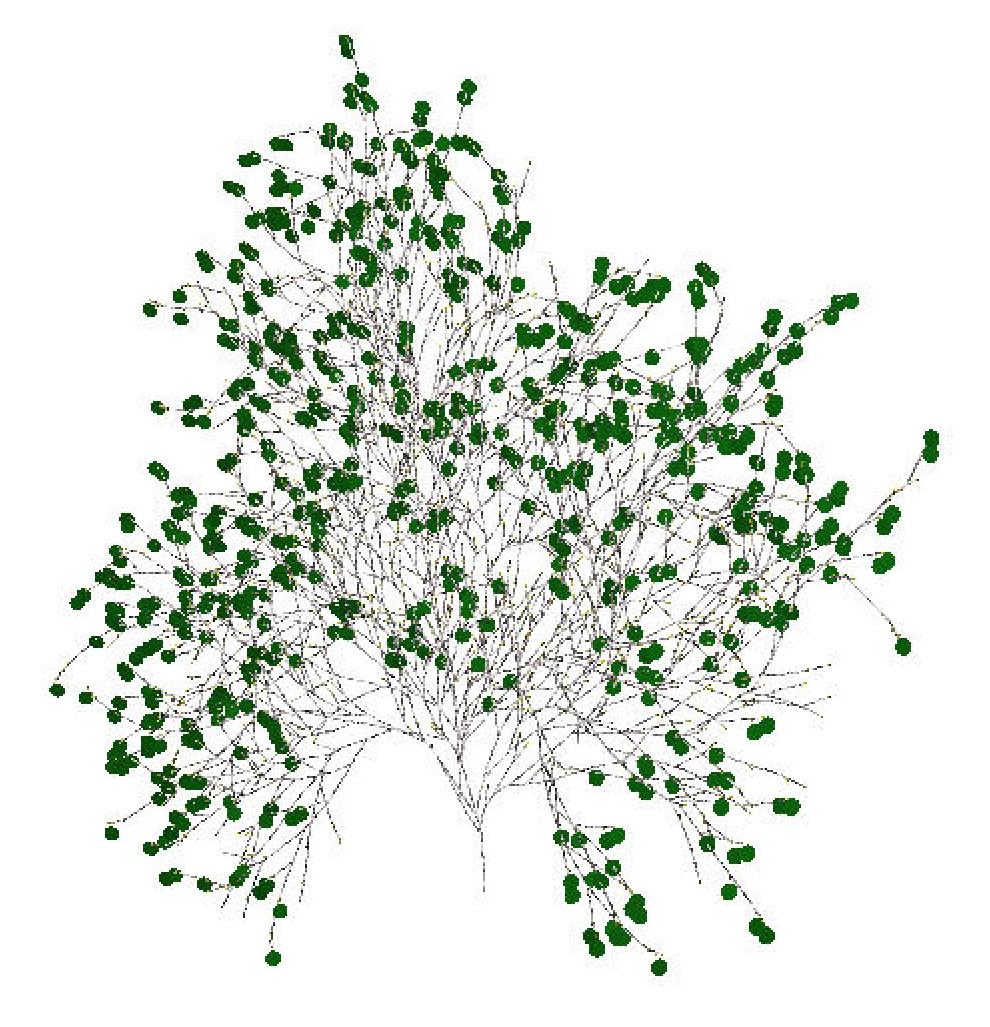
\includegraphics[scale=0.2]{a-uvaursi-15-35-30}
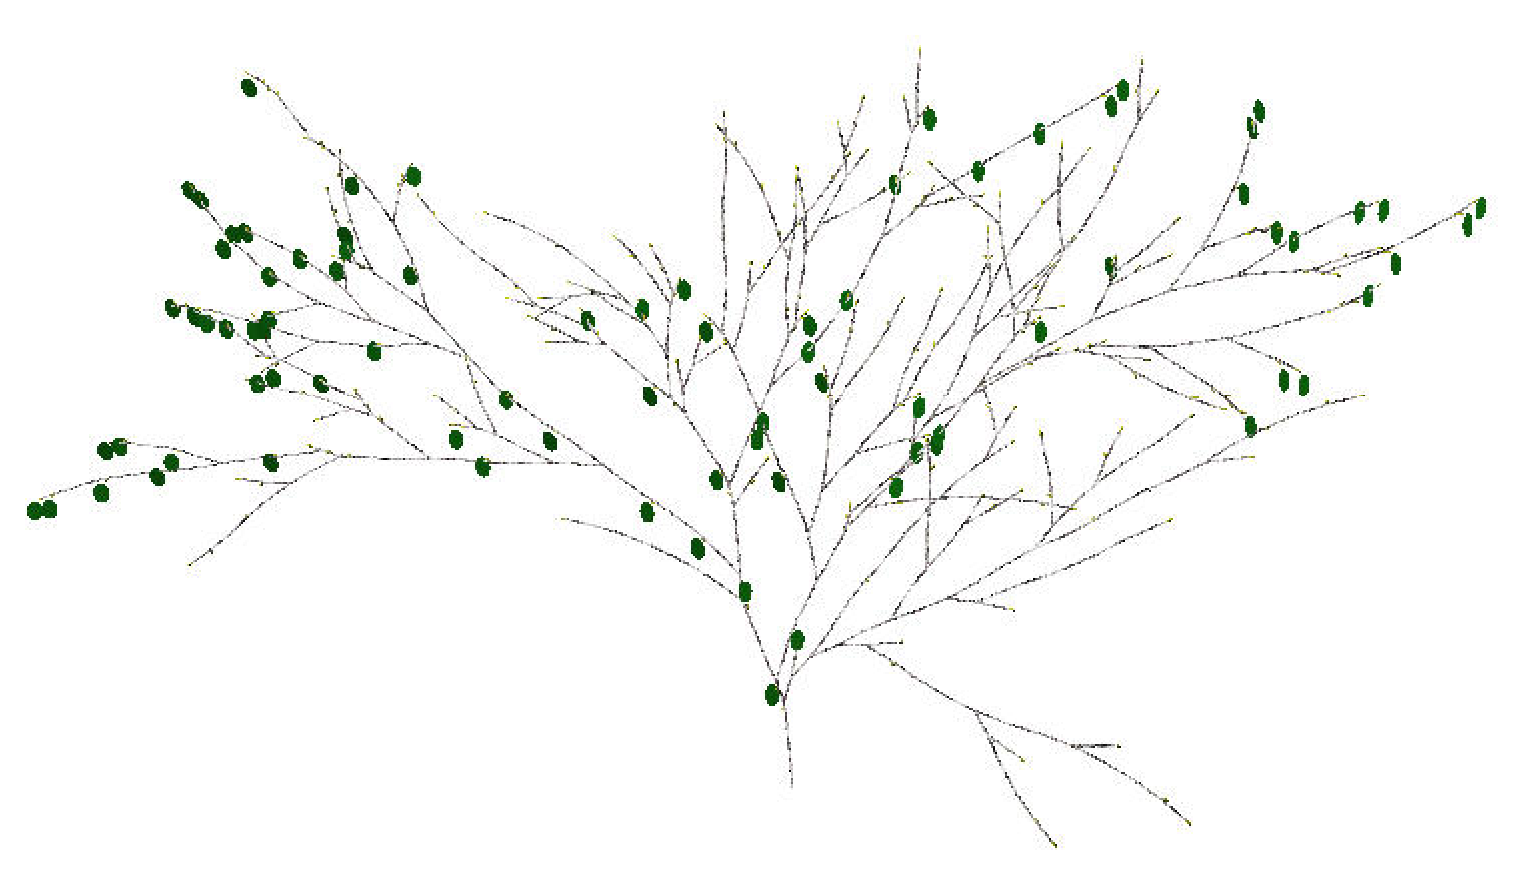
\includegraphics[scale=0.2]{a-uvaursi-15-55-30}
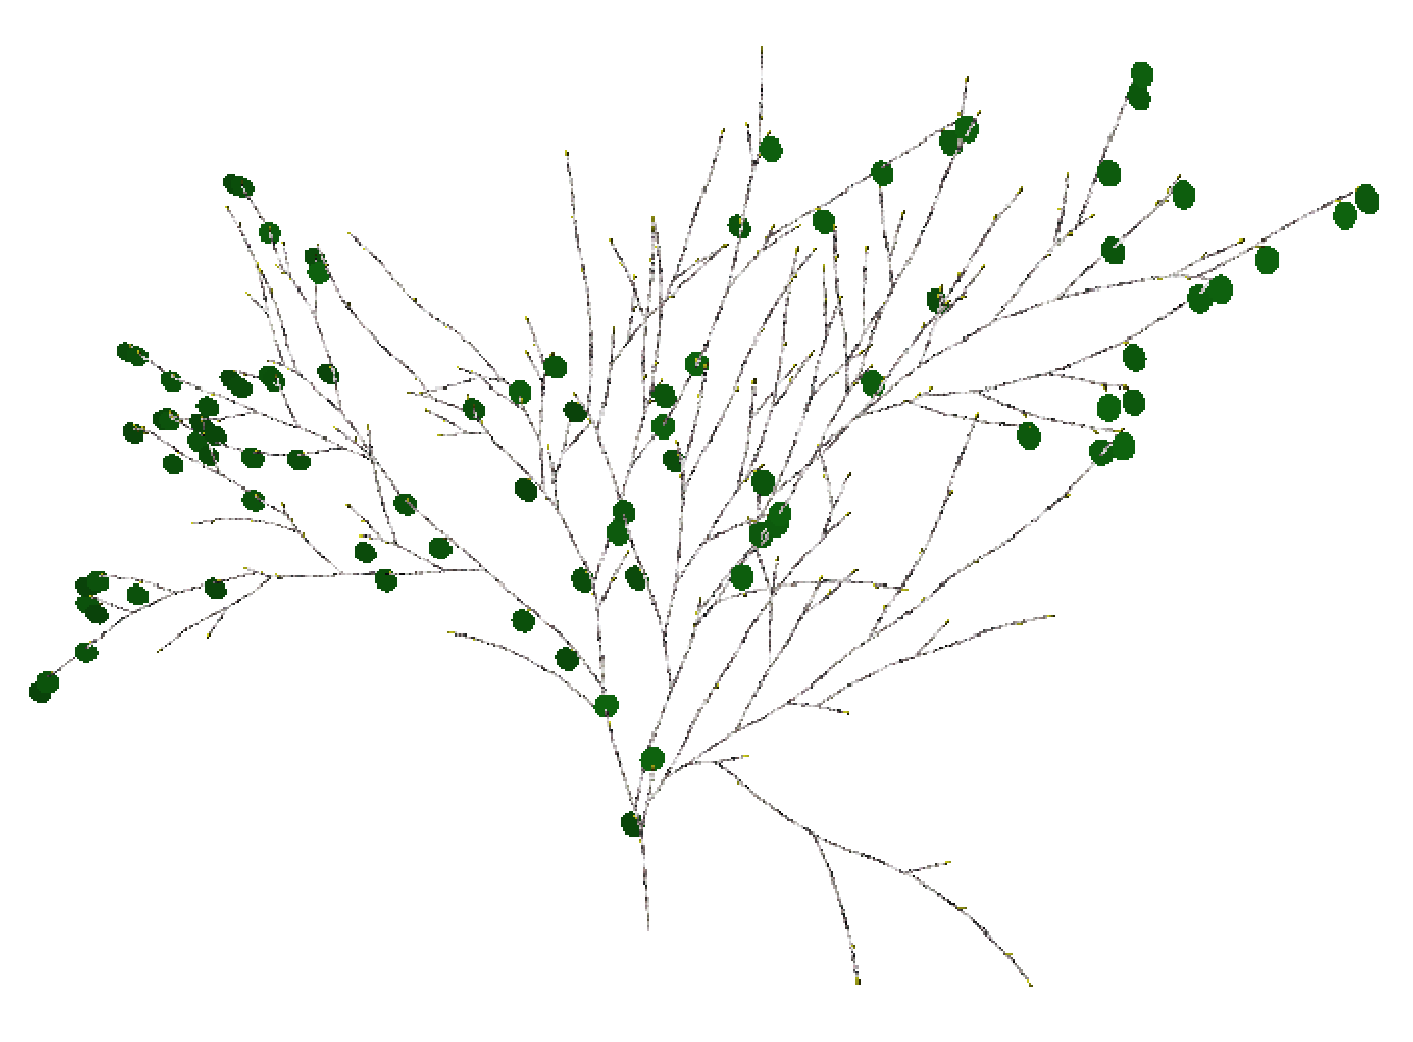
\includegraphics[scale=0.2]{a-uvaursi-15-65-30}    
\caption{Bearberry model after 15 iterations. From left to right 
  opening angle and the distance to obstacle are $35^{\circ}/30\mathrm{cm}, 
 55^{\circ}/30\mathrm{cm}$ and $65^{\circ}/20\mathrm{cm}$.}\label{fig:a-uva-ursi} 
\end{figure}
